%
% main.tex
%
% Copyright (C) 2021 by SpaceLab.
%
% Flatsat Platfor Documentation
%
% This work is licensed under the Creative Commons Attribution-ShareAlike 4.0
% International License. To view a copy of this license,
% visit http://creativecommons.org/licenses/by-sa/4.0/.
%

%
% \brief Main file.
%
% \author Gabriel Mariano Marcelino <gabriel.marcelino@spacelab.ufsc.br>
% \author Yan Castro de Azeredo <yan.azeredo@spacelab.ufsc.br>
%
% \institution Universidade Federal de Santa Catarina (UFSC)
%
% \version 0.1.0
%
% \date 2020/07/16
%

\documentclass[a4paper,12pt]{book}

\usepackage{spacelab_book}

\title{Flatsat Platform Documentation}
\author{SpaceLab}
\date{\today}

% File metadata
\hypersetup
{
    pdfauthor   = {SpaceLab},
    pdfsubject  = {\thetitle},
    pdftitle    = {\thetitle},
    pdfkeywords = {Nanosatellites, CubeSats, Testbench, Flatsat}
}

\begin{document}

    \pagenumbering{roman}
    \setcounter{page}{1}

    %
% titlepage.tex
%
% Copyright (C) 2021 by SpaceLab.
%
% Flatsat Platform Documentation
%
% This work is licensed under the Creative Commons Attribution-ShareAlike 4.0
% International License. To view a copy of this license,
% visit http://creativecommons.org/licenses/by-sa/4.0/.
%

%
% \brief Title page.
%
% \author Gabriel Mariano Marcelino <gabriel.marcelino@spacelab.ufsc.br>
%
% \institution Universidade Federal de Santa Catarina (UFSC)
%
% \version 0.2.0
%
% \date 2020/07/16
%

\begin{titlepage}

\thispagestyle{empty}

\begin{flushleft}
SLB-FLATSAT-DOC-v0.2
\end{flushleft}

\vspace{1cm}

\begin{figure}[!ht]
    \begin{flushleft}
        
\includegraphics[width=7cm]{figures/spacelab_logo_full_color_rgb_1000px_72ppi.png}
    \end{flushleft}
\end{figure}

\begin{flushleft}
\Huge{\textbf{\thetitle}}
\rule[0pt]{\textwidth}{5pt}
\end{flushleft}

\vspace{0.2cm}

\begin{flushleft}
\textit{\thetitle} \\
\textit{SpaceLab, Universidade Federal de Santa Catarina, Florianópolis - Brazil}
\end{flushleft}

\vfill
\vfill

\begin{flushright}
June 2021
\end{flushright}

\end{titlepage}

    \cleardoublepage
    %
% authorpage.tex
%
% Copyright (C) 2021 SpaceLab.
%
% Flatsat Platform Documentation
%
% This work is licensed under the Creative Commons Attribution-ShareAlike 4.0
% International License. To view a copy of this license,
% visit http://creativecommons.org/licenses/by-sa/4.0/.
%

%
% \brief Author page.
%
% \author Gabriel Mariano Marcelino <gabriel.marcelino@spacelab.ufsc.br>
%
% \institution Universidade Federal de Santa Catarina (UFSC)
%
% \version 0.1.0
%
% \date 2020/07/16
%

\thispagestyle{empty}

\begin{center}

\textbf{\thetitle}

\textit{January, 2021}

\vspace{1cm}

\textbf{Project Chief:}

Eduardo Augusto Bezerra

\vspace{1cm}

\textbf{Authors:}

Yan Castro de Azeredo \\

\vspace{1cm}

\textbf{Contributing Authors:}

Gabriel Mariano Marcelino \\
André Martins Pio de Mattos \\

\vspace{1cm}


\textbf{Revision Control:}

\end{center}

\begin{table}[!ht]
    \begin{center}
        \begin{tabular}{cL{5cm}L{5.5cm}C{2cm}}
            \toprule[1.5pt]
            \textbf{Version} & \textbf{Author}  & \textbf{Changes}    & \textbf{Date} \\
            \midrule
            0.0     & G. M. Marcelino           & Document creation   & 2020/10/11 \\
            0.1     & Y. C. de Azeredo          & First release       & 2021/01/04 \\
                    &                           &                     &            \\
                    &                           &                     &            \\
            \bottomrule[1.5pt]
        \end{tabular}
    \end{center}
\end{table}

\vfill

\begin{figure}[!h]
	\begin{center}
		
\includegraphics[width=0.25\textwidth]{figures/by-sa.pdf}
	\end{center}
\end{figure}

\textcopyright\  2021 by SpaceLab. \thetitle. This work is licensed under the Creative Commons Attribution-ShareAlike 4.0 International License. To view a copy of this license, visit \href{http://creativecommons.org/licenses/by-sa/4.0/}{http://creativecommons.org/licenses/by-sa/4.0/}.

    \cleardoublepage

    \listoffigures
    \addcontentsline{toc}{chapter}{List of Figures}

    \listoftables
    \addcontentsline{toc}{chapter}{List of Tables}

    \printnomenclature
    \addcontentsline{toc}{chapter}{Nomenclature}

    \tableofcontents
    \cleardoublepage
    
    \pagenumbering{arabic}
    \setcounter{page}{1}

    %
% introduction.tex
%
% Copyright (C) 2020 by SpaceLab.
%
% Flatsat Platform Documentation
%
% This work is licensed under the Creative Commons Attribution-ShareAlike 4.0
% International License. To view a copy of this license,
% visit http://creativecommons.org/licenses/by-sa/4.0/.
%

%
% \brief Introduction chapter.
%
% \authors: Gabriel Mariano Marcelino <gabriel.marcelino@spacelab.ufsc.br> and Yan Castro de Azeredo <yan.azeredo@spacelab.ufsc.br>
%
% \institution Universidade Federal de Santa Catarina (UFSC)
%
% \version 0.1.1
%
% \date 2020/07/16
%

\chapter{Introduction} \label{ch:introduction}

The SpaceLab FlatSat Platform is a testbed for CubeSat PCB modules. FlatSats enable easier, faster and a secure method for testing subsystens indenpently while been integrated in a flat design before going to integration on a CubeSat form factor. The PCB can support up to 7 modules, all PC104 pins are interligated to flexibilize its use, only the particularity connection between modules need to be be taken into account. One PC104 has inverted pinout, the board also makes it possible to have two seperate power supplies, a UART to USB converter for four modules, kill-switches activation though SPDTs, Remove Before Flight pin header and a connector for charging batteries. This project is to be used on the GOLDS-UFSC mission \cite{golds-ufsc} during test phase.

\begin{figure}[!ht]
    \begin{center}
        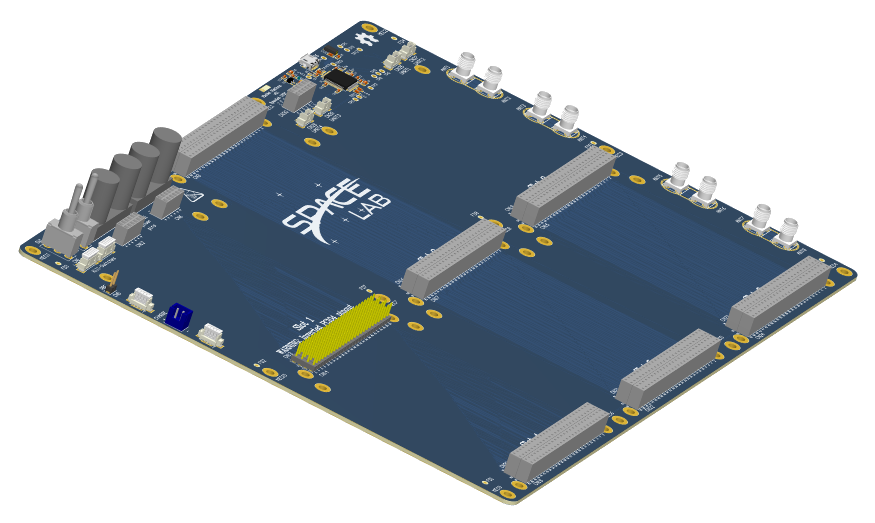
\includegraphics[width=0.75\textwidth]{figures/flatsat_perspective_image.png}
        \caption{3D view of the FlatSat PCB.}
        \label{fig:pcb-3d}
    \end{center}
\end{figure}

All the project, source and documentation files are available freely on a GitHub repository \cite{interface-board-repo} under its respective licenses.
    %
% system_overview.tex
%
% Copyright (C) 2020 by SpaceLab.
%
% Flatsat Platform Documentation
%
% This work is licensed under the Creative Commons Attribution-ShareAlike 4.0
% International License. To view a copy of this license,
% visit http://creativecommons.org/licenses/by-sa/4.0/.
%

%
% \brief System Overview chapter.
%
% \authors: Gabriel Mariano Marcelino <gabriel.marcelino@spacelab.ufsc.br> and Yan Castro de Azeredo <yan.azeredo@spacelab.ufsc.br>
%
% \institution Universidade Federal de Santa Catarina (UFSC)
%
% \version 0.1.1
%
% \date 2020/12/17
%

\chapter{System Overview} \label{ch:system-overview}

The FlatSat form factor choosen for this project is a retangular one piece design. On its current version v0.1 the platform can be purelly used hardware wise. The hardware block diagram can be seen on figure \ref{fig:block-diagram}. The PC104 slot Nº7 is supossed to be used for a extra interface, shield or another FlatSat platform.

\section{Block Diagram}

\begin{figure}[!ht]
    \begin{center}
        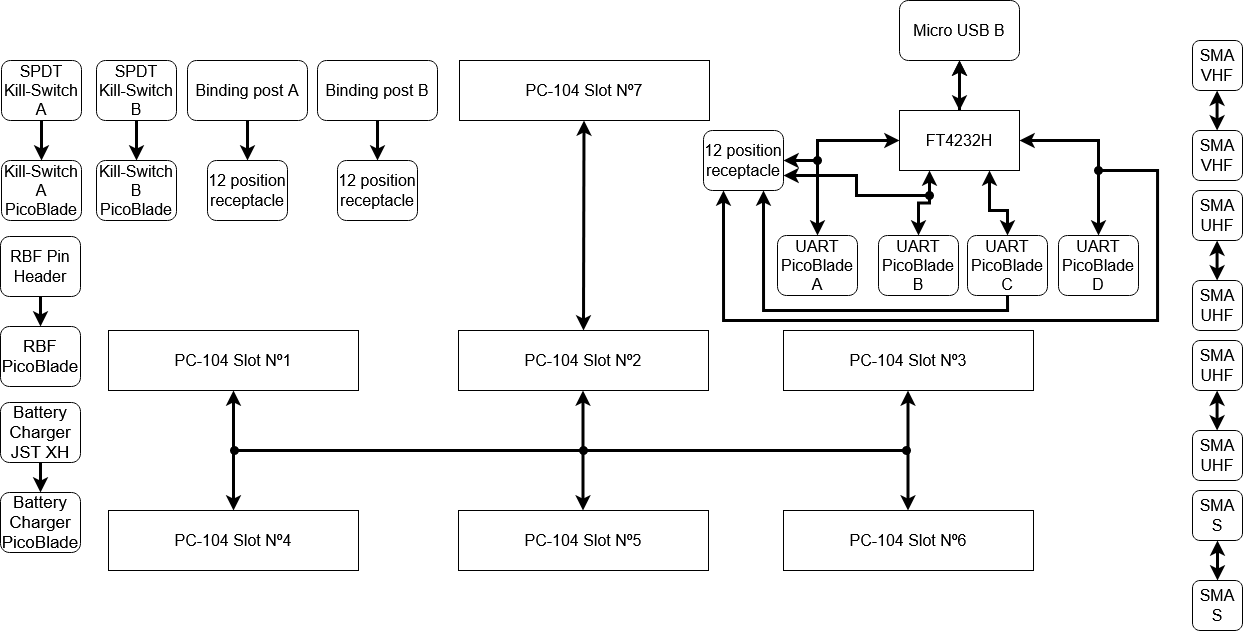
\includegraphics[width=\textwidth]{figures/flatsat_block_diagram.png}
        \caption{FlatSat hardware block diagram.}
        \label{fig:block-diagram}
    \end{center}
\end{figure}

\section{Board Dimensions}

The board is a retangular PCB with linear dimensions of 300mmx220mm. The full mechanical specs of the platform can be seen on its draftsman document available at it's GitHub repository \cite{flatsat-draftsman}.
    %
% hardware.tex
%
% Copyright (C) 2021 by SpaceLab.
%
% Flatsat Platform Documentation
%
% This work is licensed under the Creative Commons Attribution-ShareAlike 4.0
% International License. To view a copy of this license,
% visit http://creativecommons.org/licenses/by-sa/4.0/.
%

%
% \brief Hardware chapter.
%
% \author Gabriel Mariano Marcelino <gabriel.marcelino@spacelab.ufsc.br>
% \author Yan Castro de Azeredo <yan.azeredo@spacelab.ufsc.br>
%
% \institution Universidade Federal de Santa Catarina (UFSC)
%
% \version 0.2.0
%
% \date 2020/10/11
%

\chapter{Hardware} \label{ch:hardware}

This chapter describes all the FlatSat's hardware interfaces in detail. On Figures \ref{fig:pcb-top} and \ref{fig:pcb-bottom} are displayed de top and bottom PCB prints.

\begin{figure}[!ht]
    \begin{center}
        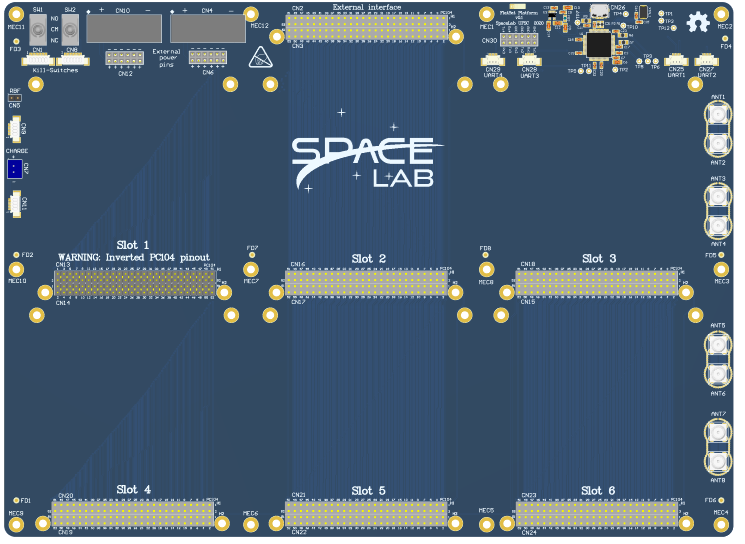
\includegraphics[width=0.8\textwidth]{figures/flatsat_top_image.png}
        \caption{FlatSat top PCB print.}
        \label{fig:pcb-top}
    \end{center}
\end{figure}

\begin{figure}[!ht]
    \begin{center}
        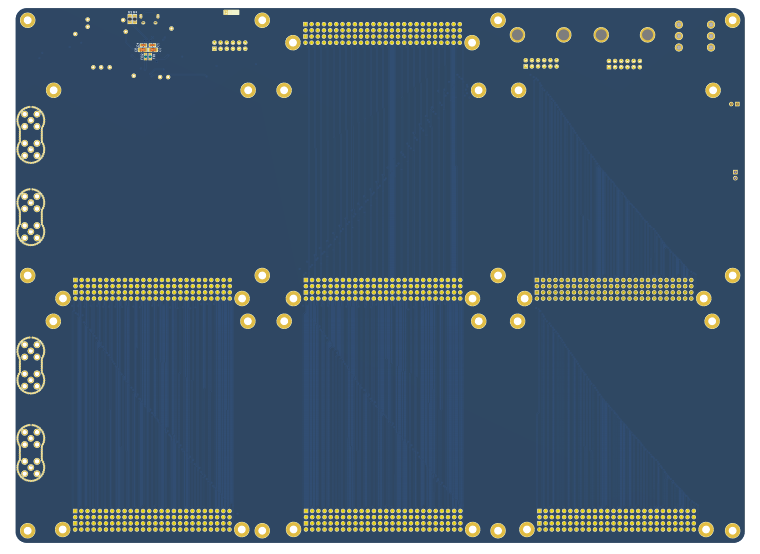
\includegraphics[width=0.8\textwidth]{figures/flatsat_bottom_image.png}
        \caption{FlatSat bottom PCB print.}
        \label{fig:pcb-bottom}
    \end{center}
\end{figure}

\section{PC-104 Interfaces}

On SpaceLab's FlatSat Platform the PC-104 interfaces are composed by two 52 pins with 2.54 mm (0.1 inch) pitch connectors. Slots N$^{\circ}$2 to N$^{\circ}$7 has two \textit{SSW-126-01-G-D} and the slot N$^{\circ}$1 uses two \textit{TSW-126-07-G-D} connectors with inverted pinout, see Figures \ref{fig:n2-n7-slots} and \ref{fig:n1-slot}. All pins are interconected to flexiblesize the positioning of the modules on the platform. All slots have grounded unlabeled mounting holes for the modules, the labeled MEC1 to MEC12 holes are for the FlatStats stability feet.

\begin{figure}[!ht]
    \begin{center}
        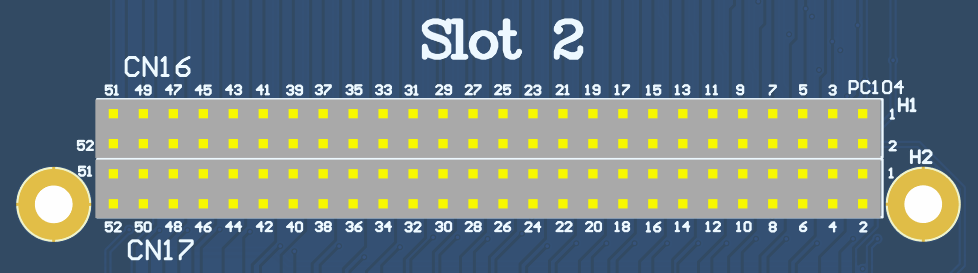
\includegraphics[width=0.75\textwidth]{figures/pc104_slots_n2_to_n7.png}
        \caption{FlatSat N$^{\circ}$2 PC-104 slot.}
        \label{fig:n2-n7-slots}
    \end{center}
\end{figure}

\begin{figure}[!ht]
    \begin{center}
        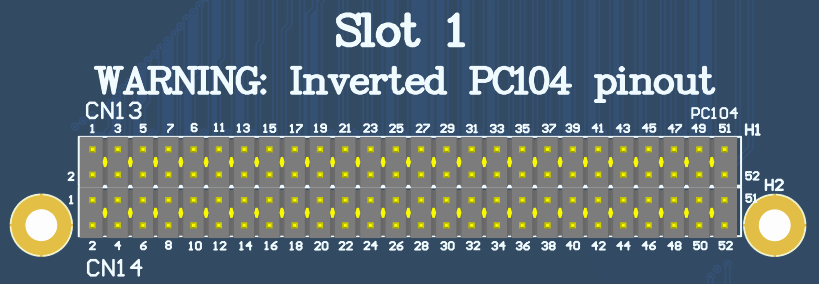
\includegraphics[width=0.75\textwidth]{figures/pc104_slot_n1.png}
        \caption{FlatSat N$^{\circ}$1 PC-104 slot.}
        \label{fig:n1-slot}
    \end{center}
\end{figure}

\section{Binding Posts and Power Receptacles}

Two sets of binding posts (\textit{4243-0}) can be mouted on the labeled CN4 and CN10 hole pads to be used for two external power supplies, see \autoref{fig:binding-posts}. The modules are powered via external jumper wires to the 12 position receptacle connectors (\textit{BCS-106-L-D-TE}) labeled CN6 and CN12. On the silkscreen the plus (+) signs are the positive power pins while the minus (-) signs are the GND pins.

\begin{figure}[!ht]
    \begin{center}
        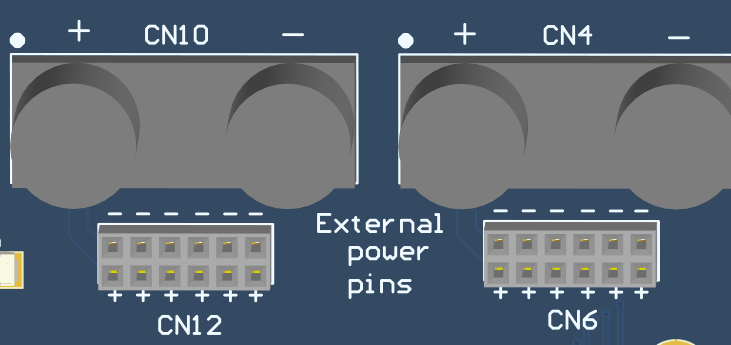
\includegraphics[width=0.75\textwidth]{figures/binding_posts.png}
        \caption{FlatSat binding posts and power receptables.}
        \label{fig:binding-posts}
    \end{center}
\end{figure}

\section{Charge Header}

On the board there is a JST XH 2 position header (\textit{B2B-XH-A-M(LF)(SN)}) for charging batteries, it can be seen in \autoref{fig:charge-connectors}. The component can suport up to 3000 mA of current, but it is advised to be used with less than 1500 mA. The 4 pin PicoBlade is to be connected to the EPS\nomenclature{\textbf{EPS}}{\textit{Electric Power System.}} module to make the interconnection for the JST header. The charge header also provides a detent lock for fastening and avoid a mistankenly reverse connection.

\begin{figure}[!ht]
    \begin{center}
        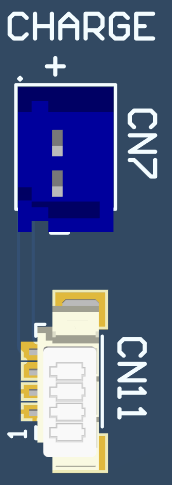
\includegraphics[width=0.15\textwidth]{figures/charge_connectors.png}
        \caption{FlatSat charge connectors.}
        \label{fig:charge-connectors}
    \end{center}
\end{figure}

\section{RBF Pin Header}

The platform has a RBF pin header that can seen \autoref{fig:rbf-connectors}. The interconnection between the header and the EPS module is done by a 4 pin PicoBlade.

\begin{figure}[!ht]
    \begin{center}
        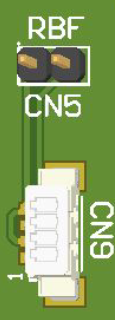
\includegraphics[width=0.15\textwidth]{figures/rbf_connectors.png}
        \caption{FlatSat RBF connectors.}
        \label{fig:rbf-connectors}
    \end{center}
\end{figure}

\section {SPDT Kill-Switches}

The kill-switches uses SPDT switches (\textit{100SP1T1B4M2QE}) for powering off the EPS module, see \autoref{fig:kill-switches-connectors}. The power off states are seen on \autoref{fig:kill-switches-states}, they are also present on the hardware schematics. The SPDTs are interconnected to the EPS module via two 6 pin PicoBlade connectors labeled CN1 and CN8.

\begin{figure}[!ht]
    \begin{center}
        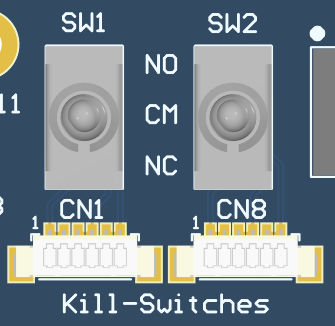
\includegraphics[width=0.5\textwidth]{figures/kill_switches_connectors.png}
        \caption{FlatSat kill-switches connectors.}
        \label{fig:kill-switches-connectors}
    \end{center}
\end{figure}

\begin{figure}[!ht]
    \begin{center}
        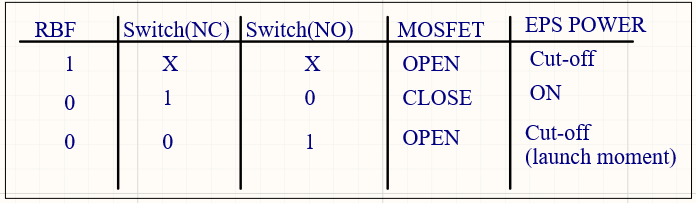
\includegraphics[width=0.75\textwidth]{figures/kill_switches_states.png}
        \caption{FlatSat kill-switches states.}
        \label{fig:kill-switches-states}
    \end{center}
\end{figure}

\section{Antenna Interfaces}

\subsection{SMA connectors}

On the PCB there are SMA connectors (\textit{132134-15}) labeled ANT1 to ANT8 for connecting VHF\nomenclature{\textbf{VHF}}{\textit{Very High Frequency.}}, UHF\nomenclature{\textbf{UHF}}{\textit{Ultra High Frequency.}} and S-Band antennas, see \autoref{fig:antennas-smas}. The receiver (RX) antenna is to be connected to one of the SMA, while the transmitter (TX) goes to the other connector and to the CubeSat module. The impedance control (see \autoref{fig:rf-track-width-calc}) and power dissipation (see \autoref{fig:rf-track-width-power-calc}) where approximately calculated for all 3 bands. As the FlatSat platform is to be used in light testing the aproximations where considered acceptable for the project.

\begin{figure}[!ht]
    \begin{center}
        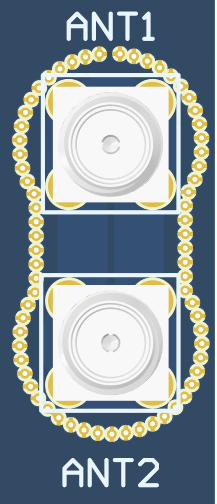
\includegraphics[width=0.15\textwidth]{figures/antennas_smas.png}
        \caption{FlatSat SMA connectors.}
        \label{fig:antennas-smas}
    \end{center}
\end{figure}

\subsection{Impedance Control of the RF Tracks}

\begin{figure}[!ht]
    \begin{center}
        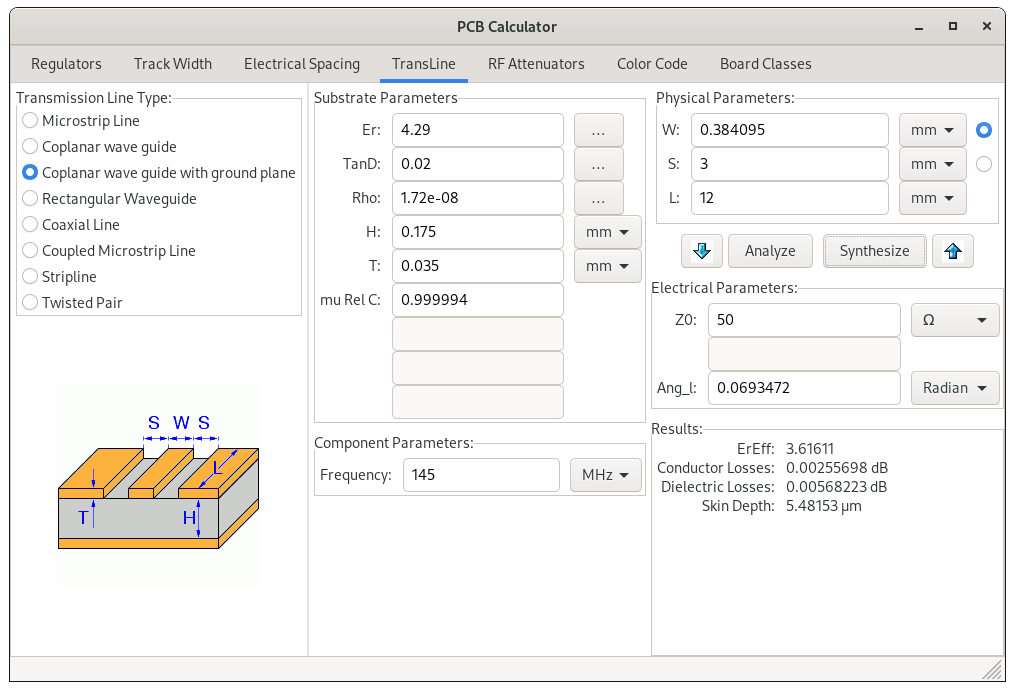
\includegraphics[width=\textwidth]{figures/rf-track-width.png}
        \caption{Calculation of the width of the RF tracks.}
        \label{fig:rf-track-width-calc}
    \end{center}
\end{figure}

\begin{figure}[!ht]
    \begin{center}
        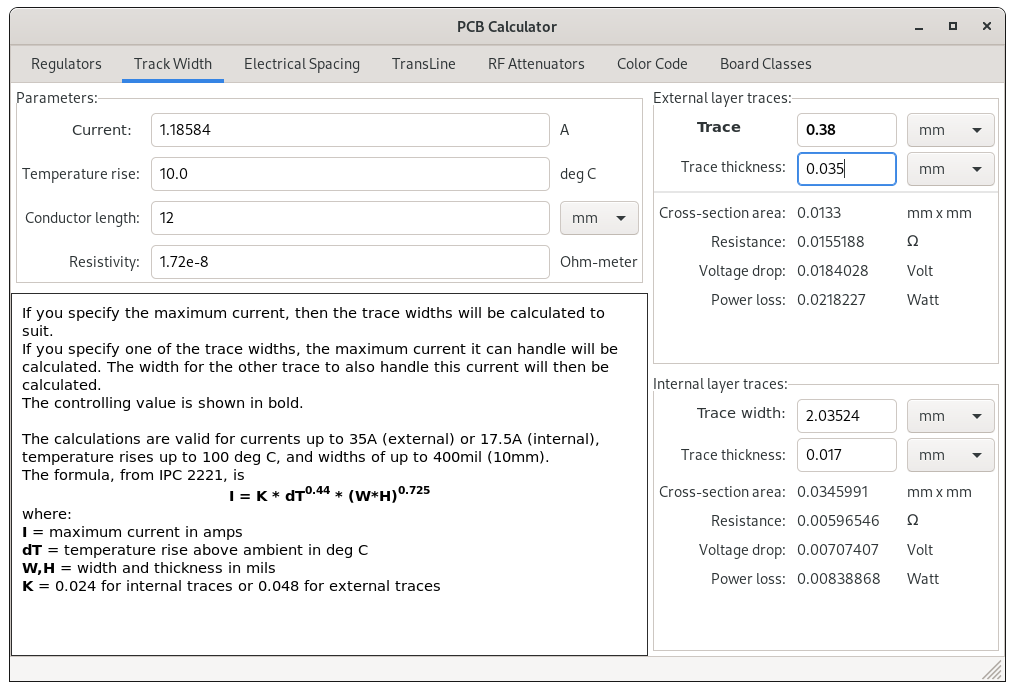
\includegraphics[width=\textwidth]{figures/rf-track-width-power.png}
        \caption{Power dissipation of the RF tracks.}
        \label{fig:rf-track-width-power-calc}
    \end{center}
\end{figure}

\section{UART to USB Converter}

There is a UART to USB converter circuit built-in the FlatSat platform for debbuging pourposes for four independent modules, it can be seen on \autoref{fig:ft4232h-circuit}. The subcircuit is self powered from a USB cable connecting a computer to a micro USB type B port (\textit{10118194-0001LF}). The USB Bridge converter IC\nomenclature{\textbf{IC}}{\textit{Integrated Circuit.}} is the \textit{FT4232HL-REEL} from FTDI. PicoBlade connectors are used for connecting the IC to the modules, see Figures \ref{fig:uart-picoblades-1} and \ref{fig:uart-picoblades-2}. It is also possible to use jumper wires connecting the 12 Position receptacle connector (\textit{BCS-106-L-D-TE}) labeled CN30 to the modules if PicoBlades are not used.

\begin{figure}[!ht]
    \begin{center}
        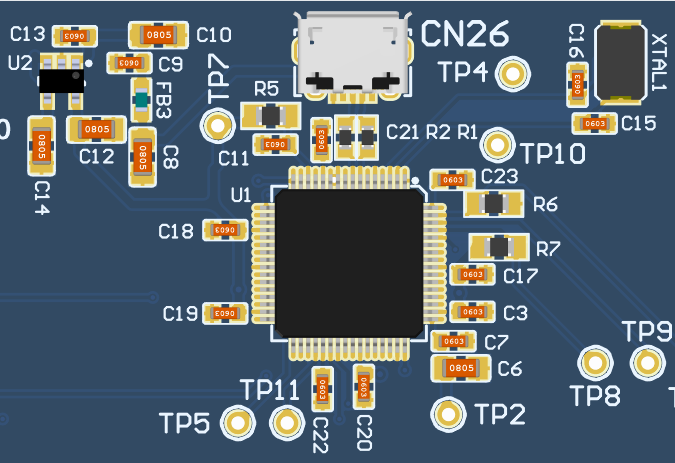
\includegraphics[width=0.75\textwidth]{figures/ft4232h_circuit.png}
        \caption{Top view of the UART to USB converter circuit.}
        \label{fig:ft4232h-circuit}
    \end{center}
\end{figure}

\begin{figure}[!ht]
    \begin{center}
        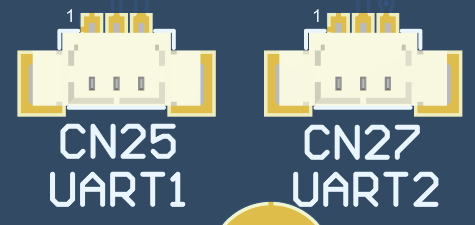
\includegraphics[width=0.5\textwidth]{figures/picoblade_uarts_n1_and_n2}
        \caption{UART PicoBlade N$^{\circ}$1 and N$^{\circ}$2 connectors.}
        \label{fig:uart-picoblades-1}
        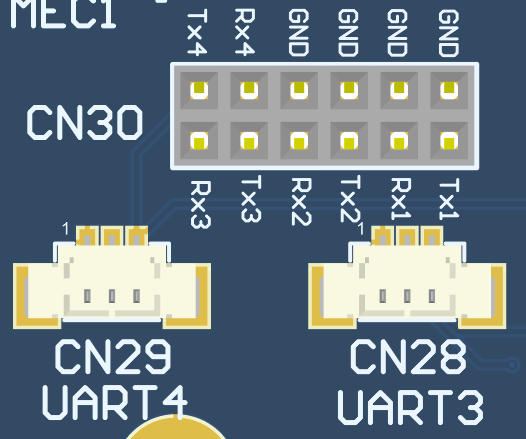
\includegraphics[width=0.5\textwidth]{figures/picoblade_uarts_n3_and_n4_and_receptable.png}
        \caption{UART PicoBlade N$^{\circ}$3 and N$^{\circ}$4 connectors and receptable.}
        \label{fig:uart-picoblades-2}
    \end{center}
\end{figure}

\section{Test Points}

The FlatSat has test points for the UART to USB converter circuit. The \autoref{tab:testpoints} displays their labels and description.

\begin{table}[!h]
    \centering
    \begin{tabular}{cllll}
        \toprule[1.5pt]
        \textit{Label} & \textit{Description} \\
        \midrule
        TP1                & (VPLL) 3V3 FT4232H power input. \\
        TP2                & (VREGOUT) 1V8 FT4232H internal power output. \\
        TP3                & (VPHY) 3V3 FT4232H power input. \\
        TP4                & (REF) Current reference for FT4232H. \\
        TP5                & (RESET\#) Reset input for FT4232H. \\
        TP6                & (EECS) EEPROM chip select - pulled down by 10k resistor. \\
        TP7                & (VCCIO) I/O interface 3V3 power supply input. \\
        TP8                & (EEDATA) EEPROM data I/O - pulled up by 10k resistor. \\
        TP9                & (EECLK) Clock signal to EEPROM - not used. \\
        TP10               & (PWREN\#) Active low power-enable output. \\
        TP11               & (SUSPEND\#) Active low when USB is in suspend mode. \\
        TP12               & (GND) 0V ground input for FT4232H.\\
        \bottomrule[1.5pt]
    \end{tabular}
    \caption{FlatSat test points.}
    \label{tab:testpoints}
\end{table}

    %
% assembly.tex
%
% Copyright (C) 2021 by SpaceLab.
%
% Flatsat Platform Documentation
%
% This work is licensed under the Creative Commons Attribution-ShareAlike 4.0
% International License. To view a copy of this license,
% visit http://creativecommons.org/licenses/by-sa/4.0/.
%

%
% \brief Board Assembly chapter.
%
% \author Gabriel Mariano Marcelino <gabriel.marcelino@spacelab.ufsc.br>
% \author Yan Castro de Azeredo <yan.azeredo@spacelab.ufsc.br>
%
% \institution Universidade Federal de Santa Catarina (UFSC)
%
% \version 0.1.0
%
% \date 2020/24/12
%

\chapter{Board Assembly}

The hardware project has the Bill of Material (BOM) avalaible at its GitHub repository in excel spreeadsheets format. The PCB can be assembled by a Pick-and-place machine using the .txt file found on the hardware/fabrication folder if desired, fiducials labeled FD\# are placed to make this possible.

\section{FlatSat Stabillity Feet}

On the PCB there are labeled MEC1 to MEC12 mouting holes on the edges and in the middle of the board to be used for stabillity feet when the board is placed on top of a test bench.

\section{DNP Components}

There is only one Do Not Place (DNP) component present in the USB to UART circuit, it is the labeled R4 pad with 0805 size (2012 metric) available for soldering the micro USB type B chassi to GND for Electromagnetic compatibility (EMC) see \autoref{fig:R4-pad}. This can be done soldering a zero-Ohm resistor for a DC path or capacitor for a high-frequency path between shield and signal ground, see section 2.2.2 of the document \cite{ftdi-usb-hardware-guidelines} for more details.

\begin{figure}[!ht]
    \begin{center}
        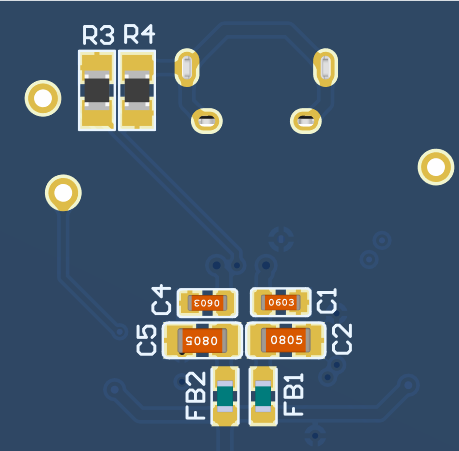
\includegraphics[width=0.5\textwidth]{figures/ft4232h_circuit_bottom.png}
        \caption{Bottom view of the UART to USB converter circuit.}
        \label{fig:R4-pad}
    \end{center}
\end{figure}

\section{Modules Mounting}

The PC-104 slots N$^{\circ}$2 to N$^{\circ}$7 are compatible for CubeSat PCB modules that are stacked in middle or the first on top. The slot N$^{\circ}$1 can only be used for the last module on this stack because of the inverted pinout. For the case of the SpaceLab's CubeSat stackup of the core modules, the last module of the stack is the EPS. For this case the EPS needs to be mounted up-side-down on slot N$^{\circ}$1 as can be seen on \autoref{fig:eps2-mouting}. For other modules any other PC-104 slots can be used, the OBDH is showed mouted on \autoref{fig:obdh2-mouting}.

\begin{figure}[!ht]
    \begin{center}
        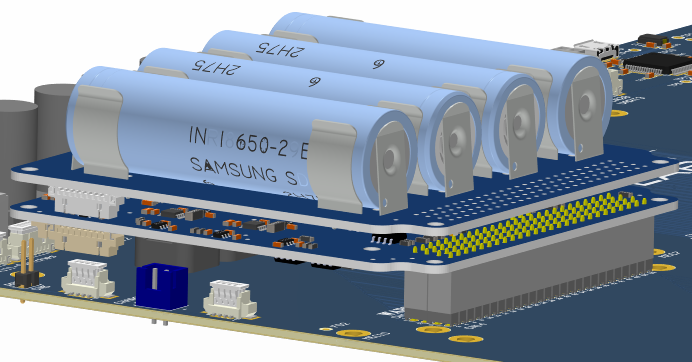
\includegraphics[width=0.8\textwidth]{figures/eps2_mouting.png}
        \caption{EPS mounted on N$^{\circ}$1 slot on a EDA tool.}
        \label{fig:eps2-mouting}
    \end{center}
\end{figure}

\begin{figure}[!ht]
    \begin{center}
        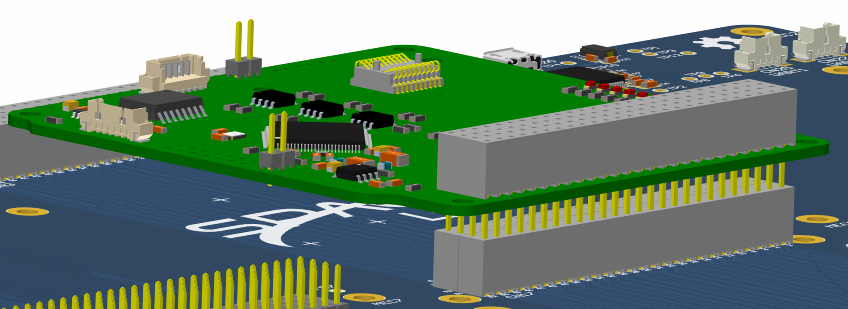
\includegraphics[width=0.8\textwidth]{figures/obdh2_mouting.png}
        \caption{OBDH mounted on N$^{\circ}$2 slot on a EDA tool.}
        \label{fig:obdh2-mouting}
    \end{center}
\end{figure}

\section{Antennas Connection}

Since the SMA connectors present on the board are on the right far side, modules placed in the opposite side may not be in reach for the connection. Because of this reason is recommended to use slots N$^{\circ}$1 and N$^{\circ}$4 for non antenna dependents PCBs.

    %
% intructions.tex
%
% Copyright (C) 2021 by SpaceLab.
%
% Flatsat Platform Documentation
%
% This work is licensed under the Creative Commons Attribution-ShareAlike 4.0
% International License. To view a copy of this license,
% visit http://creativecommons.org/licenses/by-sa/4.0/.
%

%
% \brief Usage Instructions chapter.
%
% \author Yan Castro de Azeredo <yan.azeredo@spacelab.ufsc.br>
%
% \institution Universidade Federal de Santa Catarina (UFSC)
%
% \version 0.2.0
%
% \date 2020/04/01
%

\chapter{Usage Instructions} \label{ch:instructions}

\section{Charging Batteries Through Connector}

To charge the batteries it will be needed a cable compatible with the JST XH header. The compatible housing is a XHP-2 receptacle, the jumper lead socket to socket to be used can be \textit{ASXHSXH22K305}, or any other with AWG\nomenclature{\textbf{AWG}}{\textit{American Wire Gauge.}} \#30 to \#22. The only constraint is that the current cannot excel 2000 mA, because the PicoBlades connectors used to interconnect the JST header to the EPS only supports 1000 mA per pin. For safe usage it is recommended to use the header with a maximum of 1500 mA charge current.

\section{Debugging Though USB}

Connecting a type A to micro type B USB cable to a PC\nomenclature{\textbf{PC}}{\textit{Personal Computer.}} and the USB port present on the FlatSat, the four USB to UART channels should be ready to be used. Note that the computer will recognize the port as four different devices. The FT4232H IC present on the platform  doesn't have an EEPROM\nomenclature{\textbf{EEPROM}}{\textit{Electrically-Erasable Programmable Read-Only Memory.}}, so it will be already configured to operate as default serial ports. The FT4232H will have the built-in default VID (0403) and PID (6011).

\section{Debugging Though PC-104}

Since all PC-104 interfaces are interconnected any slot can be used for probing and debbuging. Intentionally the slot N$^{\circ}$7 or also labeled ``external interface'' on the PCB was meant to be used for testing all pins. A new board or another FlatSat platform can be connected to this interface if the pinout of the specific project is compatible. The GOLDS-UFSC pinout is avalaible at its github repository \cite{golds-ufsc}.

    %
% intgration.tex
%
% Copyright (C) 2021 by SpaceLab.
%
% Flatsat Platform Documentation
%
% This work is licensed under the Creative Commons Attribution-ShareAlike 4.0
% International License. To view a copy of this license,
% visit http://creativecommons.org/licenses/by-sa/4.0/.
%

%
% \brief Modules Integration and Testing chapter.
%
% \author João Cláudio Elsen Barcellos <joaoclaudiobarcellos@gmail.com>
%
% \institution Universidade Federal de Santa Catarina (UFSC)
%
% \version 0.2.0
%
% \date 2021/06/15
%

\chapter{Modules Integration and Testing} \label{ch:modules-integration-and-testing}

The CubeSat that will be used in the FloripaSat-2 consists mainly of three modules, OBDH, TTC and EPS, which are the core of the CubeSat, and payloads. In order to facilitate the integration and testing of all these subsystems a methodology had to be created, which will be done using the FlatSat platform.

This process was divided in five steps, which will be presented in the next sections with more details. First, the core of the CubeSat will be connected together, to evaluate the interaction between them. Then, the GRS will be emulated to verify if there will be no errors in data transmission and reception. Later, all payloads will be connected together with the core of the CubeSat to evaluate their behavior. Next the the GRS will be emulated again with the core and payloads integrated, considering the data transmission from the payloads. Finally, a long term test will be made.

\section{Testing the CubeSat Core}

In this step, the interaction between OBDH, EPS and TTC will be evaluated. Therefore, the main communication protocols that these three modules use to interact will be tested. The deployment sequence will be performed with a fully functional EPS and also with a partially functional EPS, to search for critical errors. Subsequently, the operation of these modules will be evaluated.

\subsection{Experiment Setup}
\label{subsec:experiment-setup-1}

First, all three modules will be connected to the FlatSat. The EPS needs to be connected to \textbf{Slot 1}, and the other two modules can be connected in any slots, like in figure \ref{fig:connections-1}.

\begin{figure}[H]
	\begin{center}
		
\includegraphics[width=0.5\textwidth]{figures/dummy-image.png}
		\caption{OBDH, EPS and TTC connected in the FlatSat platform.}
		\label{fig:connections-1}
	\end{center}
\end{figure}

Still with the kill-switches cutting-off the power supply for the EPS, a power supply is connected to the Battery Module, like in figure \ref{fig:connections-2}. But, if the EPS won't be used in the experiment, OBDH and TTC can be powered by using an external power supply connected to the binding posts CN10 or CN4. Jumpers are used to connect their respective PC-104 power supply pins to CN12 or CN6, like in figure \ref{fig:connections-3}. 

\begin{figure}[H]
	\begin{center}
		
\includegraphics[width=0.5\textwidth]{figures/dummy-image.png}
		\caption{Setup using the EPS and Battery Module.}
		\label{fig:connections-2}
	\end{center}
\end{figure}

\begin{figure}[H]
	\begin{center}
		
\includegraphics[width=0.5\textwidth]{figures/dummy-image.png}
		\caption{Setup without the EPS and Battery Module.}
		\label{fig:connections-3}
	\end{center}
\end{figure}

A launchpad will emulate the antennas, like the MSP-EXP430F5529LP. Then, this launchpad can be connected in the \textbf{Slot 7}, so OBDH and TTC can communicate with it, like in figure \ref{fig:connections-4}.

\begin{figure}[H]
	\begin{center}
		
\includegraphics[width=0.5\textwidth]{figures/dummy-image.png}
		\caption{Launchpad emulating the Antenna Module.}
		\label{fig:connections-4}
	\end{center}
\end{figure}

\subsection{Deployment Sequence}

After the decouple of the satellite from its deployer in orbit, the kill-switches will be released and will enable the power supply of the core modules. The EPS will distribute energy for all subsystems, with the Battery Module coupled, composed by four lithium-ion 18650 cells. After the boot, OBDH waits 45 minutes before operating normally. Then, the OBDH will act to deploy the antennas. Similarly to the ODBH, after de boot, TTC waits 55 minutes before operating normally. Redundantly, the TTC will also act to deploy the antennas. The TTC will enable the sub-modules Downlink/Uplink and Beacon at the end of the process. Every 12 hours, this process repeats, indefinitely, but the OBDH and TTC don’t need to wait anymore to operate normally. The figure \ref{fig:deployment-flowchart} shows the process described.

\begin{figure}[H]
	\begin{center}
		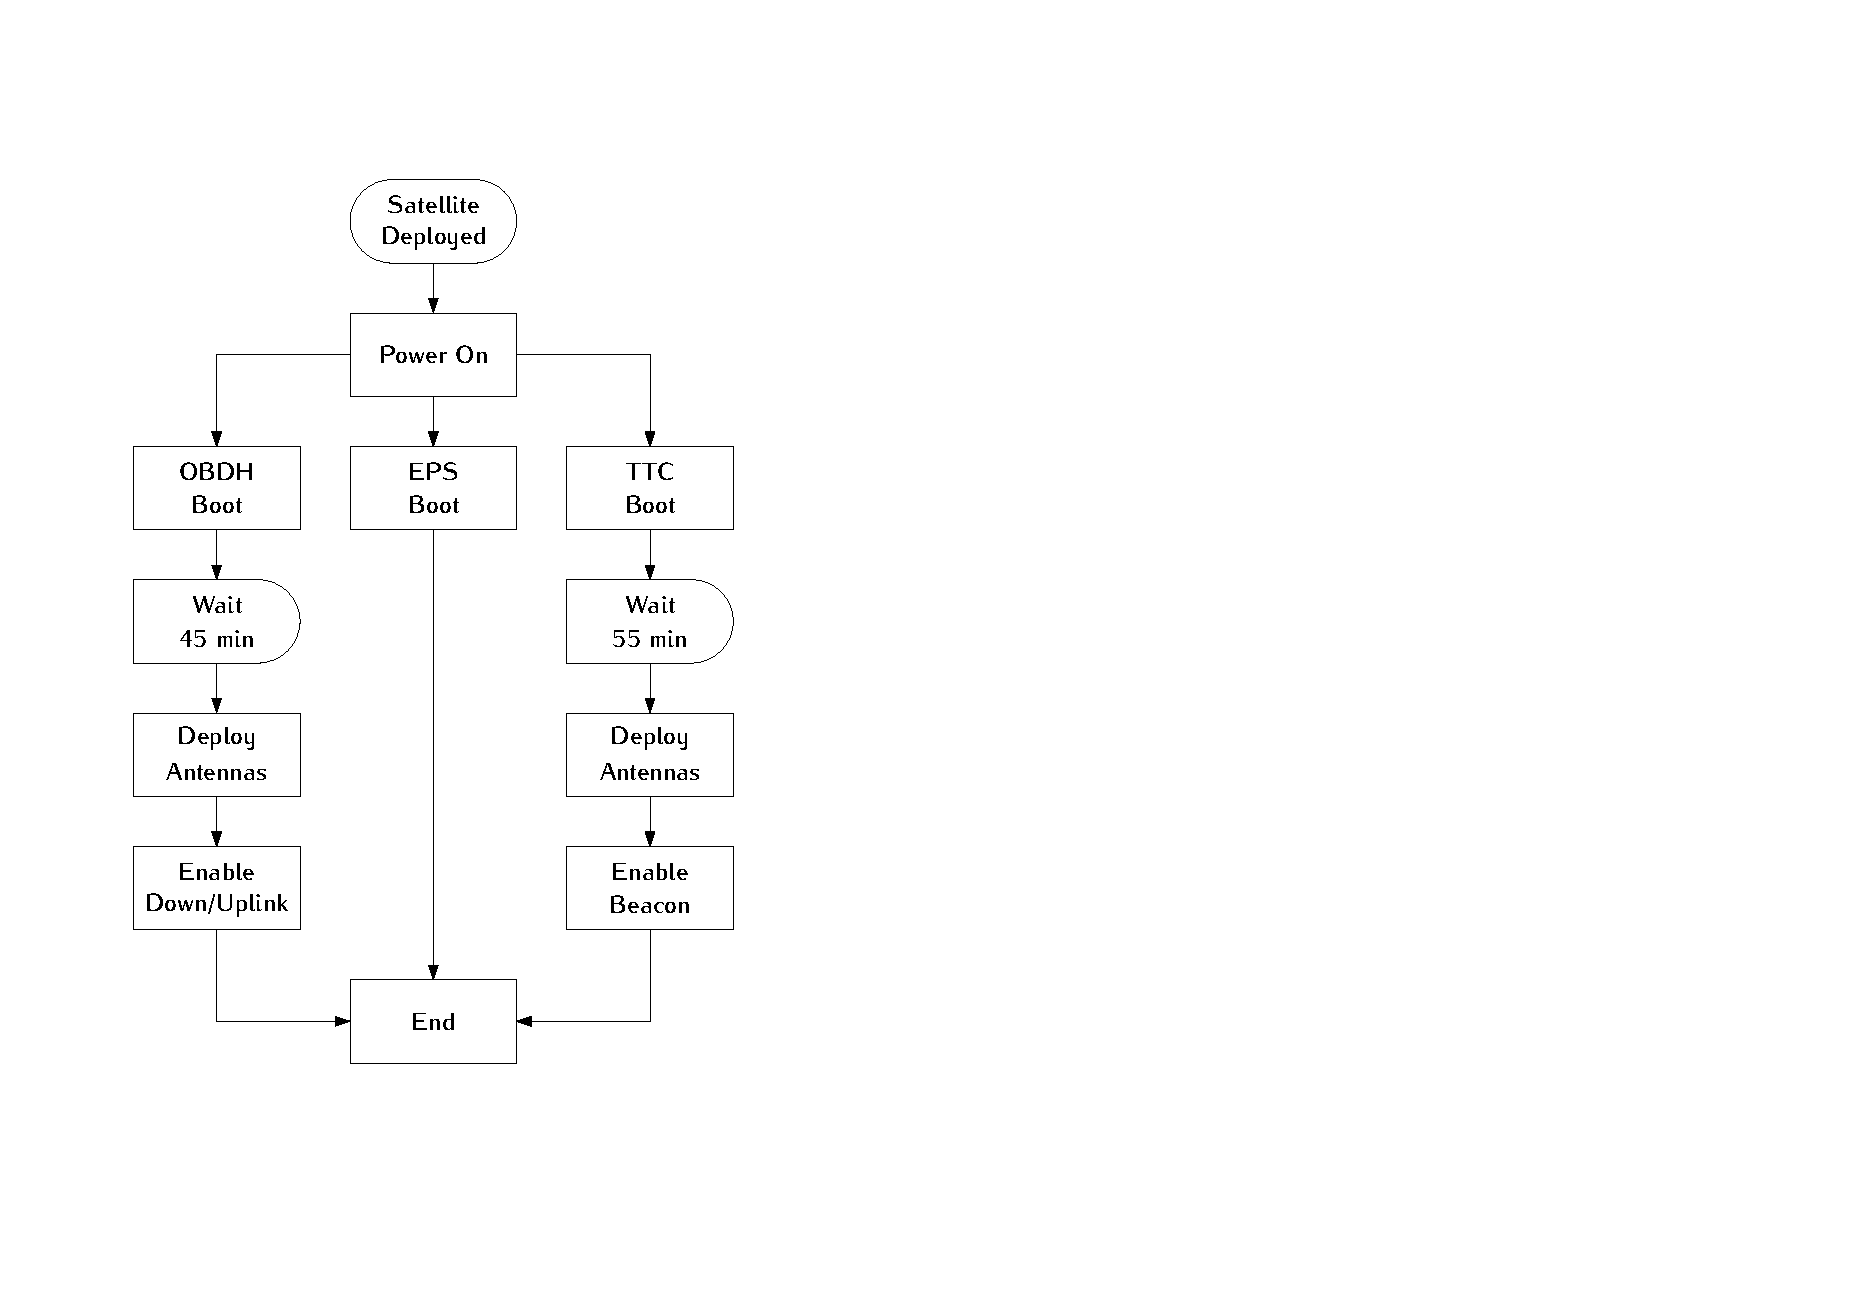
\includegraphics[width=0.5\textwidth]{figures/deployment-flowchart.pdf}
		\caption{Flowchart of the deployment sequence.}
		\label{fig:deployment-flowchart}
	\end{center}
\end{figure}

\subsubsection{Waiting Time and Redudancy}

The OBDH and TTC won’t operate normally for 45 minutes and 55 minutes, respectively. The validation criteria for this first experiment is shown in the table \ref{tab:validation-criteria-1}.

\begin{table}[H]
	\centering
	\resizebox{\columnwidth}{!}{\begin{tabular}{cc}
		\toprule[1.5pt]
		\textit{Question} & \textit{Answer} \\
		\midrule
		Is the OBDH doing something before 45 minutes?  & No, 45 minutes elapsed before the OBDH act to deploy the antennas. \\
		Is the TTC doing something before 55 minutes? & No, 55 minutes elapsed before the TTC act to deploy the antennas. \\
		\bottomrule[1.5pt]
	\end{tabular}}
	\caption{Validation criteria.}
	\label{tab:validation-criteria-1}
\end{table}

Then, OBDH and TTC, respectively, will act to deploy the antennas. The validation criteria for this first experiment is shown in the table \ref{tab:validation-criteria-2}.

\begin{table}[H]
	\centering
	\resizebox{\columnwidth}{!}{\begin{tabular}{cc}
			\toprule[1.5pt]
			\textit{Question} & \textit{Answer} \\
			\midrule
			TTC was capable of doing the deployment of the antennas, like the OBDH? & Yes, OBDH and TTC were capable of doing the same thing.\\
			\bottomrule[1.5pt]
	\end{tabular}}
	\caption{Validation criteria.}
	\label{tab:validation-criteria-2}
\end{table}

\subsubsection{Power Supply}

The EPS uses the MPPT, a method used to distribute energy with more efficiency. But, if the EPS cannot implement this method, theoretically, still would be able to distribute the energy to the other modules, but with less efficiency. But, to guarantee, this need to be evaluated. The validation criteria for this first experiment are shown in the table \ref{tab:validation-criteria-3}.

\begin{table}[H]
	\centering
	\resizebox{\columnwidth}{!}{\begin{tabular}{cc}
			\toprule[1.5pt]
			\textit{Question} & \textit{Answer} \\
			\midrule
			If the EPS fails to implement the MPPT, OBDH and TTC will boot? & Yes, OBDH and TTC booted.\\
			\bottomrule[1.5pt]
	\end{tabular}}
	\caption{Validation criteria.}
	\label{tab:validation-criteria-3}
\end{table}

\subsection{Interactions}

After the deployment sequence, during 12 hours, the satellite works normally. Therefore, the modules will get all the relevant data for the mission. This data flows between modules, via UART, SPI and $I^{2}C$. These interactions need to be evaluated to understand if the data is traveling correctly, with no faults. 

\subsubsection{Interaction between TTC and EPS}

The sub-module Beacon interacts with the EPS using the UART. Every one minute the EPS will receive a request, from the sub-module Beacon, to send data. If the data sent from the EPS is valid, the Beacon will transmit the data from the TTC itself and from the EPS. Otherwise, only the data from TTC will be transmitted. This operation is presented in figure \ref{fig:beacon-flowchart}.  

\begin{figure}[H]
	\begin{center}
		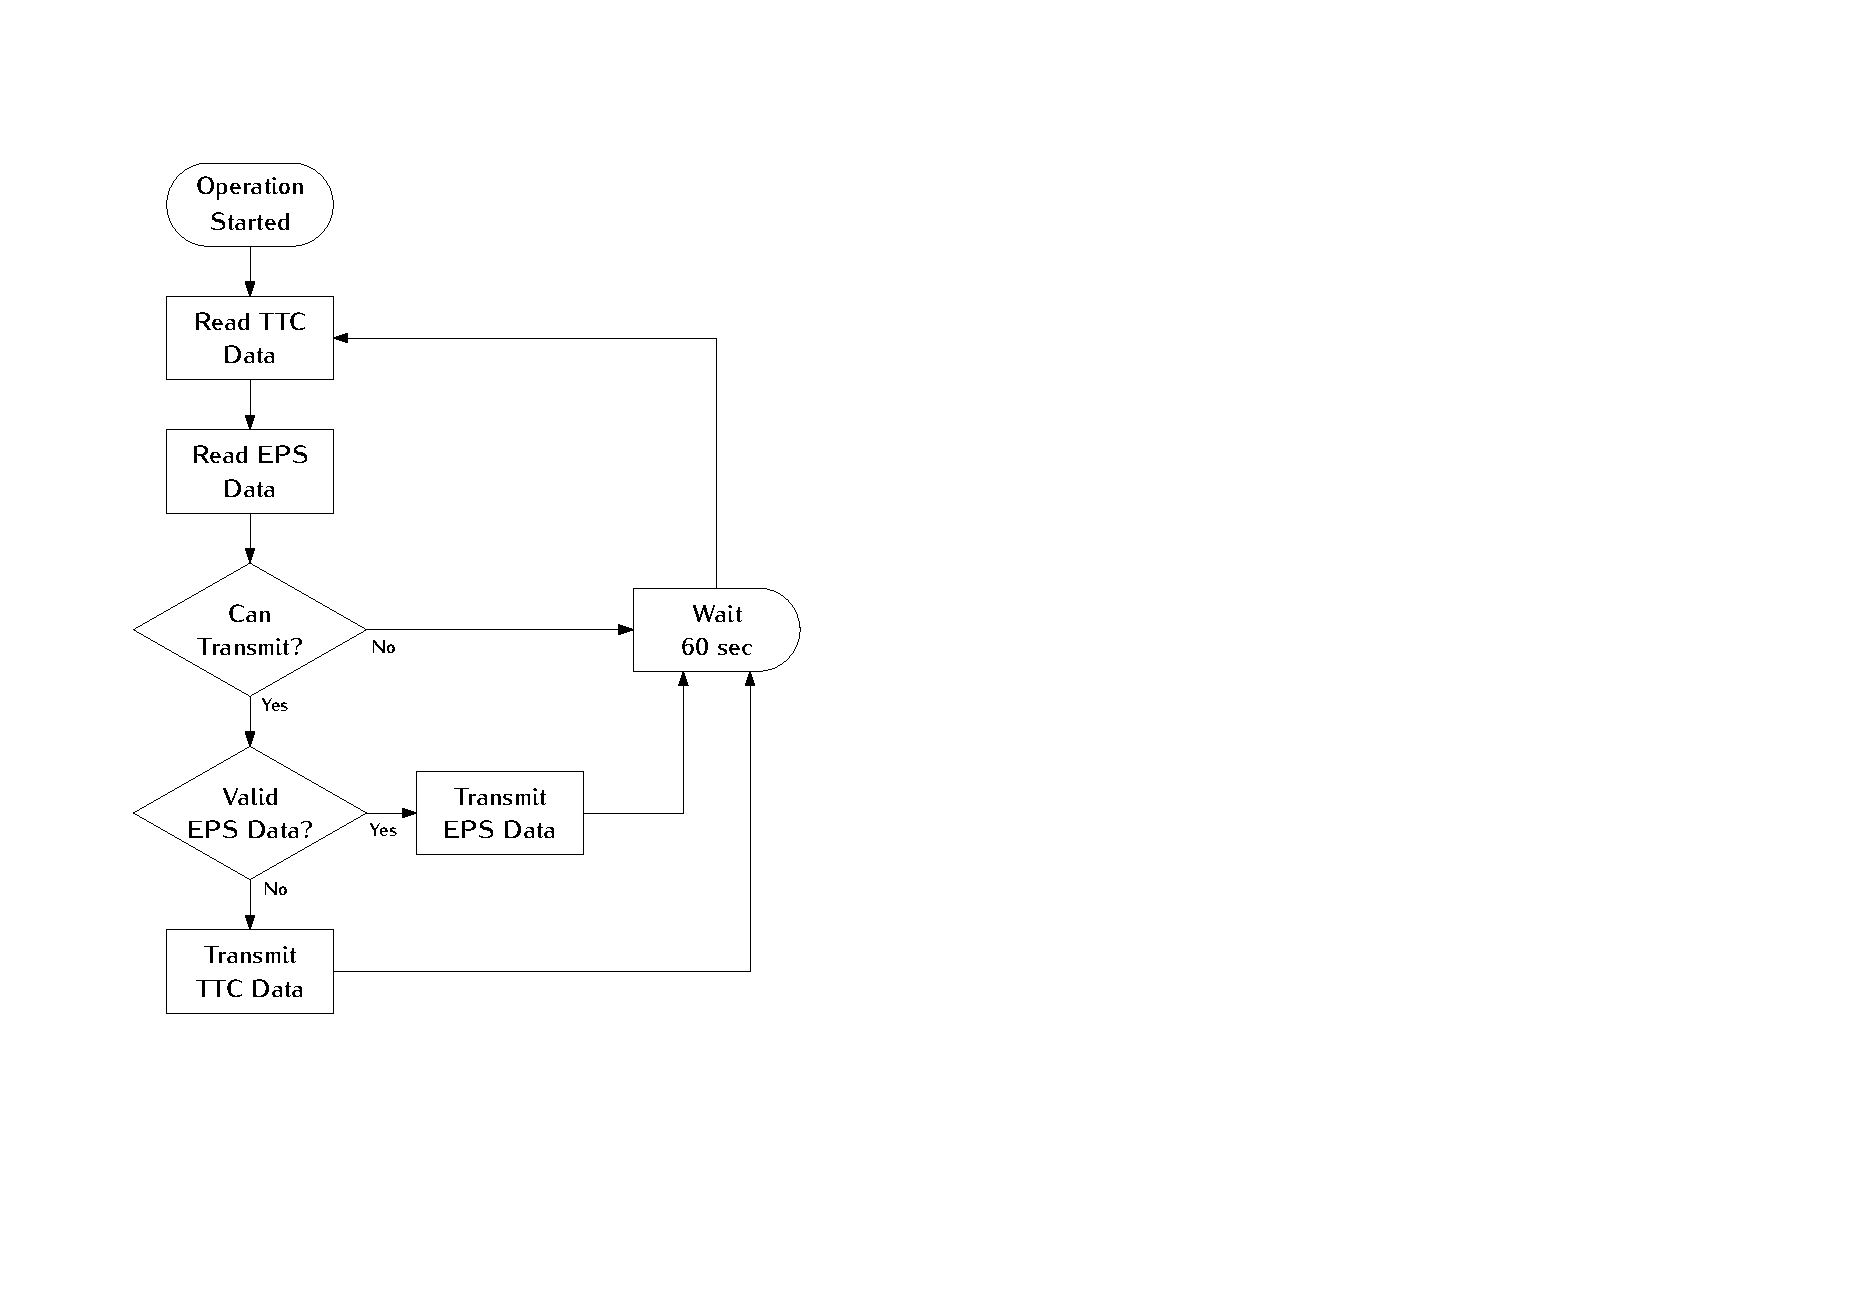
\includegraphics[width=0.5\textwidth]{figures/beacon-flowchart.pdf}
		\caption{Flowchart of the Beacon operation.}
		\label{fig:beacon-flowchart}
	\end{center}
\end{figure}

In the firmware of each module, it is calculated the checksum of every message that is transmitted or received. This way, it is possible to understand if the message sent from one module is the same that is received from the other. This will be used to validate the interaction between EPS and Beacon. The validation criteria is shown in table \ref{tab:validation-criteria-4}. 

\begin{table}[H]
	\centering
	\resizebox{\columnwidth}{!}{\begin{tabular}{cc}
			\toprule[1.5pt]
			\textit{Question} & \textit{Answer} \\
			\midrule
			EPS received the same message that was sent from Beacon? & Yes, the checksum was equal in both ends.\\
			Beacon received the same message that was sent from EPS? & Yes, the checksum was equal in both ends.\\
			If the data from EPS is invalid, just the TTC data is transmitted? & Yes, just the data from TTC is transmitted.\\
			And if it is valid, TTC and EPS data are transmitted? & Yes, both are transmitted.\\
            This interaction occurs every one minute? & Yes, this interaction is periodic.\\

			\bottomrule[1.5pt]
	\end{tabular}}
	\caption{Validation criteria.}
	\label{tab:validation-criteria-4}
\end{table}

\subsubsection{Interaction between OBDH with EPS and TTC}

The OBDH interacts with the TTC using SPI and with the EPS using $I^{2}C$. Every one minute, the EPS and TTC will receive a request, from the OBDH, to send data. Then, the OBDH will save all the received data (
including the data from the OBDH itself) in memory. This operation is presented in figure \ref{fig:obdh-flowchart}. 

\begin{figure}[H]
	\begin{center}
		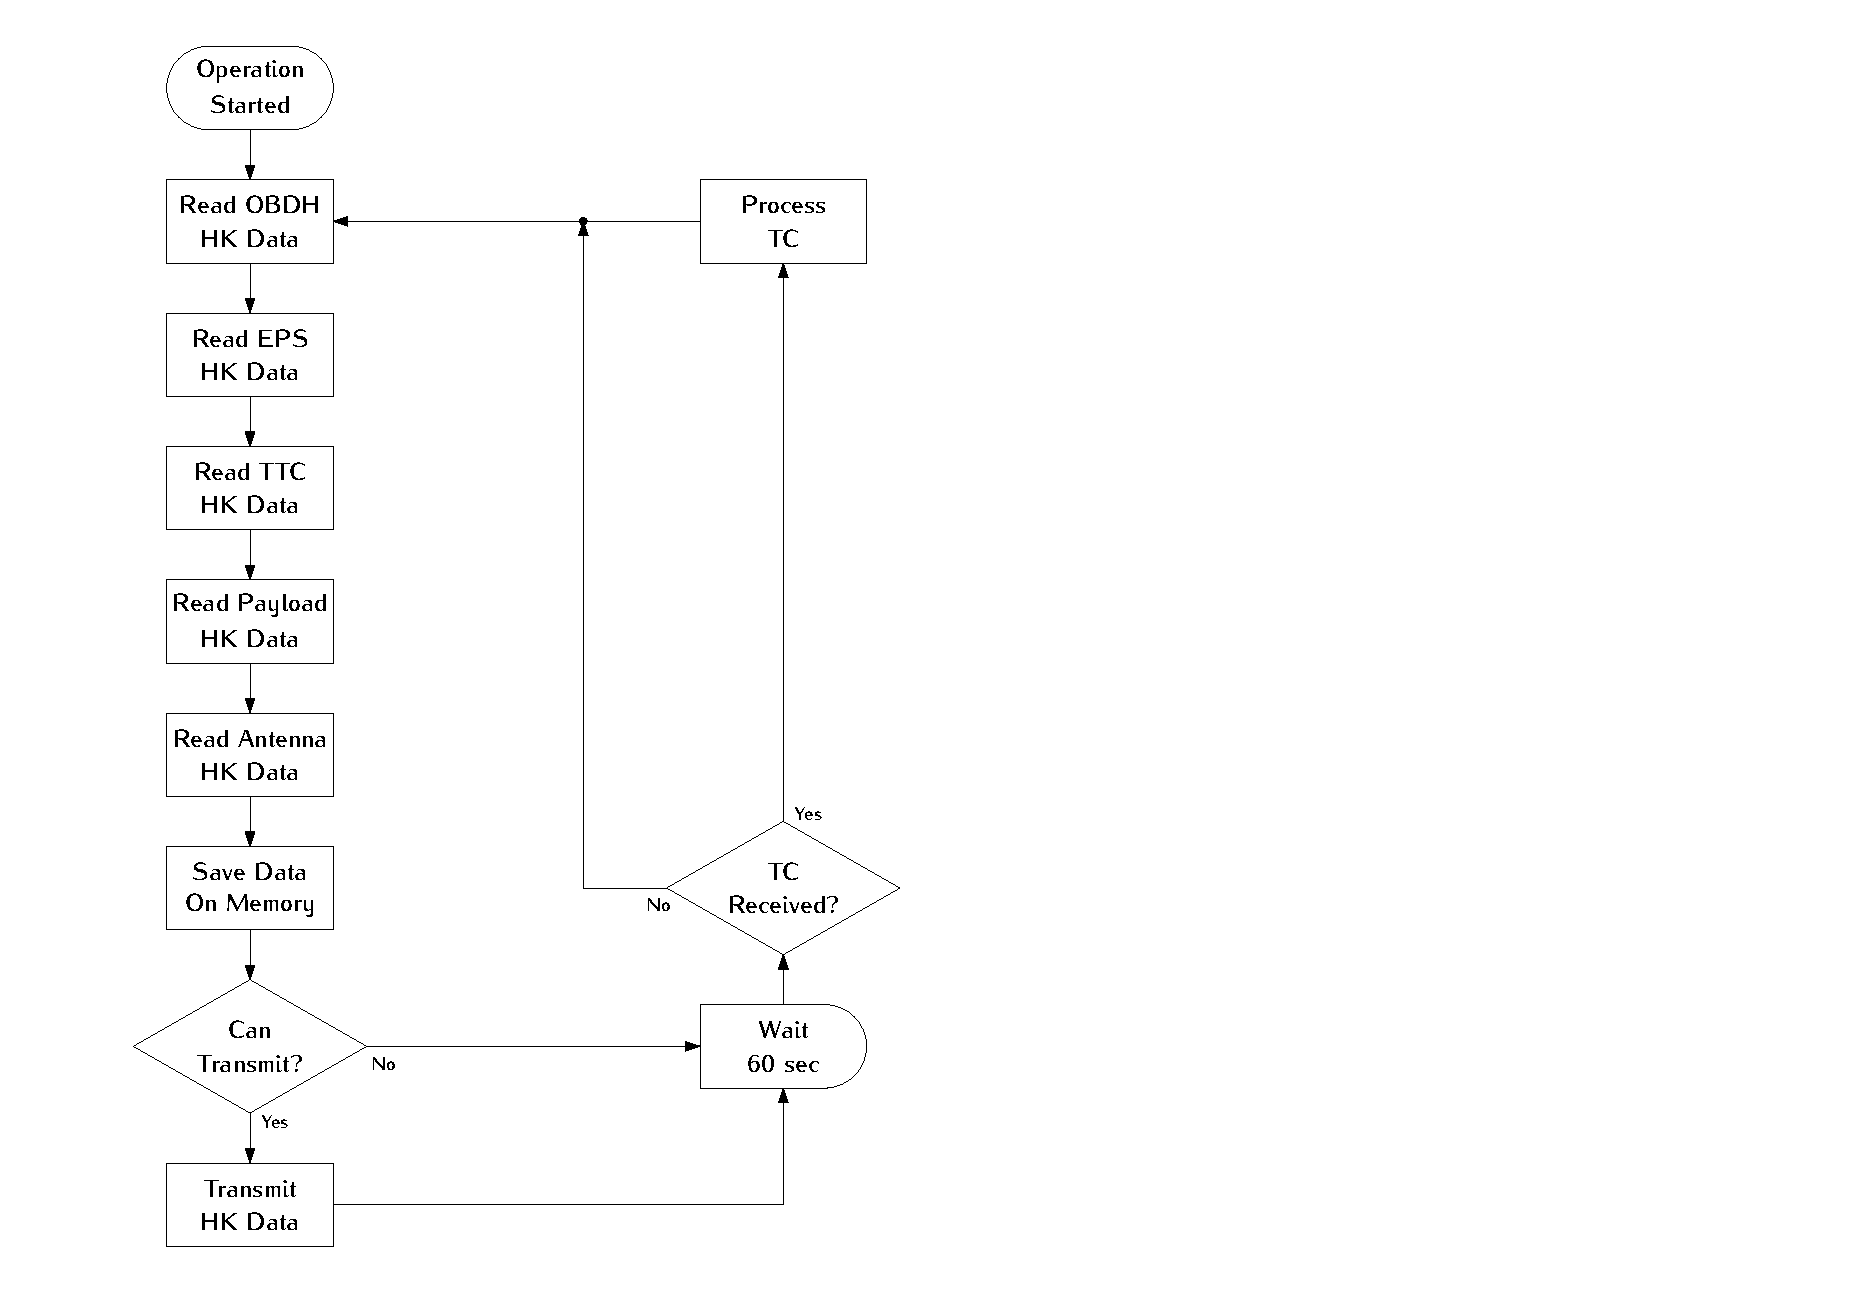
\includegraphics[width=0.5\textwidth]{figures/obdh-flowchart.pdf}
		\caption{Flowchart of the Beacon operation.}
		\label{fig:obdh-flowchart}
	\end{center}
\end{figure}

As said before, the checksum in both ends will be compared to define if the messages are being correctly sent and received. The validation criteria is shown in table \ref{tab:validation-criteria-5}.

\begin{table}[H]
	\centering
	\resizebox{\columnwidth}{!}{\begin{tabular}{cc}
			\toprule[1.5pt]
			\textit{Question} & \textit{Answer} \\
			\midrule
			EPS received the same message that was sent from OBDH? & Yes, the checksum was equal in both ends.\\
			OBDH received the same message that was sent from EPS? & Yes, the checksum was equal in both ends.\\
			TTC received the same message that was sent from OBDH? & Yes, the checksum was equal in both ends.\\
			OBDH received the same message that was sent from TTC? & Yes, the checksum was equal in both ends.\\
			OBDH was capable of saving all the data? & Yes, all data was saved in memory.\\
            This interactions occurs every one minute? & Yes, this interactions are periodic.\\

			\bottomrule[1.5pt]
	\end{tabular}}
	\caption{Validation criteria.}
	\label{tab:validation-criteria-5}
\end{table}

\section{Testing the CubeSat Core with GRS}

In this step, all the interactions between the core modules were validated. Now, the interaction of these modules with the GRS need to be evaluated. To emulate the GRS, a software, the GQRX, will be used with two boards to transmit and receive TC's, the USRP and SDR, respectively. The figure \ref{fig:tc-flowchart} shows all TC's involved.

\begin{figure}[H]
	\begin{center}
		\includegraphics[width=0.4\textwidth]{figures/tc-flowchart.pdf}
		\caption{Flowchart of the telecommand processing.}
		\label{fig:tc-flowchart}
	\end{center}
\end{figure}

\subsection{Experiment Setup}

Similarly to the subsection \ref{subsec:experiment-setup-1}, all three modules will be connected to the FlatSat. But, now, the GRS will be emulated. The USRP and the SDR should be connected to the computer, witch will be running the GQRX, like in figure \ref{fig:connections-5}.

\begin{figure}[H]
	\begin{center}
		
\includegraphics[width=0.5\textwidth]{figures/dummy-image.png}
		\caption{Setup to emulate the GRS.}
		\label{fig:connections-5}
	\end{center}
\end{figure}

\subsection{Receiving data from GRS}

As shown in figure \ref{fig:obdh-flowchart}, after OBDH saves the data in memory, it will check if TC's were received, then, it will process the TC's. In figure \ref{fig:tc-flowchart}, are listed all the TC's that can be processed. In this step, only the TC's with ID 47h, 48h, 4Bh won't be transmited by GRS, because there aren't payloads connected to the FlatSat. The sub-module Uplink has the function of receiving the TC's and inform OBDH. The GQRX will be used to configure the message that will be transmitted to the Uplink and the USRP should transmit this message to it. The validation criteria is shown in table \ref{tab:validation-criteria-6}.

\begin{table}[H]
	\centering
	\resizebox{\columnwidth}{!}{\begin{tabular}{cc}
			\toprule[1.5pt]
			\textit{Question} & \textit{Answer} \\
			\midrule
			TC with ID 40h was received? & Yes, OBDH was capable of recognising this TC.\\
			TC with ID 41h was received? & Yes, OBDH was capable of recognising this TC.\\
			TC with ID 42h was received? & Yes, OBDH was capable of recognising this TC.\\
			TC with ID 43h was received? & Yes, OBDH was capable of recognising this TC and the hibernation mode was enable.\\
			TC with ID 44h was received? & Yes, OBDH was capable of recognising this TC and the hibernation mode was disable.\\
			TC with ID 45h was received? & Yes, OBDH was capable of recognising this TC.\\
			TC with ID 46h was received? & Yes, OBDH was capable of recognising this TC.\\
			TC with ID 49h was received? & Yes, OBDH was capable of recognising this TC and the memory was erased.\\
			TC with ID 4Ah was received? & Yes, OBDH was capable of recognising this TC and the core modules was reset.\\
			\bottomrule[1.5pt]
	\end{tabular}}
	\caption{Validation criteria.}
	\label{tab:validation-criteria-6}
\end{table}

\subsection{Transmitting data to GRS}

As shown in figure \ref{fig:beacon-flowchart}, the Beacon transmits the data from the EPS and/or TTC, every one minute. The TC's 00h and 01h corresponds to the data of EPS an TTC, respectively. The SDR will receive this TC's and will be possible to see them in the GQRX. The validation criteria is shown in table \ref{tab:validation-criteria-7}.

\begin{table}[H]
	\centering
	\resizebox{\columnwidth}{!}{\begin{tabular}{cc}
			\toprule[1.5pt]
			\textit{Question} & \textit{Answer} \\
			\midrule
			TC with ID 00h was received? & Yes, the message is shown in GQRX.\\
			TC with ID 01h was received? & Yes, the message is shown in GQRX.\\
			TC's are received periodically? & Yes, the message is shown periodically in GQRX.\\
			\bottomrule[1.5pt]
	\end{tabular}}
	\caption{Validation criteria.}
	\label{tab:validation-criteria-7}
\end{table}

But, the sub-module Downlink will transmit TC's to the GRS too. For example, all the feedback transmitted to the GRS, shown in figure \ref{fig:tc-flowchart}, is transmitted by the Downlink. Also, as shown in figure \ref{fig:obdh-flowchart}, after OBDH saves the data, the Downlink will transmit a TC, with the data of all modules, every one minute. Consequently, this TC's will be shown in GQRX too. The validation criteria is shown in table \ref{tab:validation-criteria-8}.

\begin{table}[H]
	\centering
	\resizebox{\columnwidth}{!}{\begin{tabular}{cc}
			\toprule[1.5pt]
			\textit{Question} & \textit{Answer} \\
			\midrule
			In response to the TC with ID 43h, the TC with ID 25h was received? & Yes, the message is shown in GQRX.\\
			In response to the TC with ID 44h, the TC with ID 25h was received? & Yes, the message is shown in GQRX.\\
			In response to the TC with ID 45h, the TC with ID 25h was received? & Yes, the message is shown in GQRX.\\
			In response to the TC with ID 46h, the TC with ID 25h was received? & Yes, the message is shown in GQRX.\\
			In response to the TC with ID 49h, the TC with ID 25h was received? & Yes, the message is shown in GQRX.\\
			In response to the TC with ID 4Ah, the TC with ID 25h was received? & Yes, the message is shown in GQRX.\\
			In response to the TC with ID 40h, the TC with ID 21h was received? & Yes, the message is shown in GQRX.\\
			In response to the TC with ID 41h, the TC with ID 22h was received? & Yes, the message is shown in GQRX.\\
			In response to the TC with ID 42h, the TC with ID 23h was received? & Yes, the message is shown in GQRX.\\
			Every one minute a TC with ID 20h is received? & Yes, the message is shown periodically in GQRX.\\
			\bottomrule[1.5pt]
	\end{tabular}}
	\caption{Validation criteria.}
	\label{tab:validation-criteria-8}
\end{table}

    %
% references.tex
%
% Copyright (C) 2020 by SpaceLab.
%
% Flatsat Platform Documentation
%
% This work is licensed under the Creative Commons Attribution-ShareAlike 4.0
% International License. To view a copy of this license,
% visit http://creativecommons.org/licenses/by-sa/4.0/.
%

%
% \brief References chapter.
%
% \author Gabriel Mariano Marcelino <gabriel.mm8@gmail.com>
%
% \institution Universidade Federal de Santa Catarina (UFSC)
%
% \version 0.1.0
%
% \date 2020/07/16
%

\bibliography{references/test,references/obdh2}

\addcontentsline{toc}{chapter}{References}


\end{document}
